% VLDB template version of 2020-08-03 enhances the ACM template, version 1.7.0:
% https://www.acm.org/publications/proceedings-template
% The ACM Latex guide provides further information about the ACM template

\documentclass[sigconf,nonacm,pdfa,screen]{acmart}
% \settopmatter{authorsperrow=4}
% \usepackage[a-2b]{pdfx}
\usepackage{listings}
\usepackage{algorithm}
\usepackage{algpseudocode}
\usepackage{float}
% \usepackage{balance}
\floatstyle{plaintop}
\restylefloat{table}

\renewcommand{\algorithmicrequire}{\textbf{Input:}}
\renewcommand{\algorithmicensure}{\textbf{Output:}}
\renewcommand{\algorithmiccomment}[1]{\hfill \textit{// #1}}
\algtext*{EndFor}% Remove "end for" text
\algtext*{EndWhile}% Remove "end while" text
\algtext*{EndIf}% Remove "end if" text

%\usepackage{fontawesome}
\newcommand{\eg}{e.\,g.,\ }
\newcommand{\ie}{i.\,e.,\ }
\usepackage{csquotes} %\enquote{}

%% The following content must be adapted for the final version
% paper-specific
\newcommand\vldbdoi{10.14778/3648160.3648175}
\newcommand\vldbpages{1350 - 1363}
% issue-specific
\newcommand\vldbvolume{17}
\newcommand\vldbissue{6}
\newcommand\vldbyear{2024}
% should be fine as it is
\newcommand\vldbauthors{\authors}
\newcommand\vldbtitle{\shorttitle} 
% leave empty if no availability url should be set
\newcommand\vldbavailabilityurl{https://github.com/damslab/reproducibility/tree/master/vldb2024-POLAR}
% whether page numbers should be shown or not, use 'plain' for review versions, 'empty' for camera ready
\newcommand\vldbpagestyle{empty} 

\newcommand{\mat}[1]{\ensuremath{\mathbf{#1}}}
\newtheorem{example2}{Example}
\newcommand{\card}[1]{\lvert #1\rvert}

\begin{document}

\title{POLAR: Adaptive and Non-invasive Join Order Selection via Plans of Least Resistance}

%%
%% The "author" command and its associated commands are used to define the authors and their affiliations.
\author{David Justen}\authornote{Corresponding author's email: david.justen@tu-berlin.de}
\affiliation{\institution{TU Berlin}}
%\email{david.justen@tu-berlin.de}
%\orcid{1234-5678-9012}

\author{Daniel Ritter}
\affiliation{\institution{SAP}}
%\email{daniel.ritter@sap.com}
%\orcid{0000-0001-6146-3365}

\author{Campbell Fraser}
\affiliation{\institution{Google}}
%\email{campbellf@google.com}

\author{Andrew Lamb}
\author{Nga Tran}
\affiliation{\institution{InfluxData}}
%\email{{alamb,ntran}@influxdata.com}
%\email{alamb@influxdata.com}
%\email{ntran@influxdata.com}

\author{Allison Lee}
\affiliation{\institution{Snowflake}}
%\email{allison.lee@snowflake.com}

\author{Thomas Bodner}
\affiliation{\institution{Hasso Plattner Institute}\institution{University of Potsdam}}
%\email{thomas.bodner@hpi.de}
%\orcid{0000-0002-7822-2098}

\author{Mhd Yamen Haddad}
\affiliation{\institution{INRIA, Ecole Polytechnique}}
%\email{mhd-yamen.haddad@inria.fr}
%\email{mhaddad@yugabyte.com}
%\orcid{0000-0002-2206-1328}

\author{Steffen Zeuch}
\author{Volker Markl}
\affiliation{\institution{TU Berlin}}
%\email{{first.last}@tu-berlin.de}

\author{Matthias Boehm}
\affiliation{\institution{TU Berlin}}

%%
%% The abstract is a short summary of the work to be presented in the
%% article.
\begin{abstract}
%1. State the problem
Join ordering and query optimization are crucial for query performance but remain challenging due to unknown or changing characteristics of query intermediates, especially for complex queries with many joins.
%2. Say why it's an interesting problem
Over the past two decades, a spectrum of techniques for adaptive query processing (AQP)---including inter-/intra-operator adaptivity and tuple routing---have been proposed to address these challenges. However, commercial database systems in practice do not implement holistic AQP techniques because they increase the system complexity (e.g., intertwined planning and execution) and thus, complicate debugging and testing. Additionally, existing approaches may incur large overheads, leading to problematic performance regressions.
%3. Say what your solution achieves
In this paper, we introduce POLAR, a simple yet very effective technique for a self-regulating selection of alternative join orderings with bounded overhead. We enhance left-deep join pipelines with alternative join orders, perform regret-bounded tuple routing to find and validate \enquote{plans of least resistance}, and then process the majority of tuple batches through these plans. We study different join order selection techniques, different routing strategies, and a variety of workload characteristics.
%4. Say what follows from your solution
Our experiments with a POLAR prototype in DuckDB show runtime improvements of up to 9x and less than 7\% overhead for all benchmark queries, while outperforming state-of-the-art AQP systems by up to 15x.
\end{abstract}

\maketitle

%%% do not modify the following VLDB block %%
%%% VLDB block start %%%
\pagestyle{\vldbpagestyle}
\begingroup\small\noindent\raggedright\textbf{PVLDB Reference Format:}\\
\vldbauthors. \vldbtitle. PVLDB, \vldbvolume(\vldbissue): \vldbpages, \vldbyear.\\
\href{https://doi.org/\vldbdoi}{doi:\vldbdoi}
\endgroup
\begingroup
\renewcommand\thefootnote{}\footnote{\noindent
This work is licensed under the Creative Commons BY-NC-ND 4.0 International License. Visit \url{https://creativecommons.org/licenses/by-nc-nd/4.0/} to view a copy of this license. For any use beyond those covered by this license, obtain permission by emailing \href{mailto:info@vldb.org}{info@vldb.org}. Copyright is held by the owner/author(s). Publication rights licensed to the VLDB Endowment. \\
\raggedright Proceedings of the VLDB Endowment, Vol. \vldbvolume, No. \vldbissue\ %
ISSN 2150-8097. \\
\href{https://doi.org/\vldbdoi}{doi:\vldbdoi} \\
}\addtocounter{footnote}{-1}\endgroup
%%% VLDB block end %%%

%%% do not modify the following VLDB block %%
%%% VLDB block start %%%
\ifdefempty{\vldbavailabilityurl}{}{
\vspace{.3cm}
\begingroup\small\noindent\raggedright\textbf{PVLDB Artifact Availability:}\\
The source code, data, and/or other artifacts have been made available at \url{\vldbavailabilityurl}.
\endgroup
}
%%% VLDB block end %%%

%% INTRODUCTION
\section{Introduction}
\label{sec:intro}

\begin{figure*}[t]
    \centering
    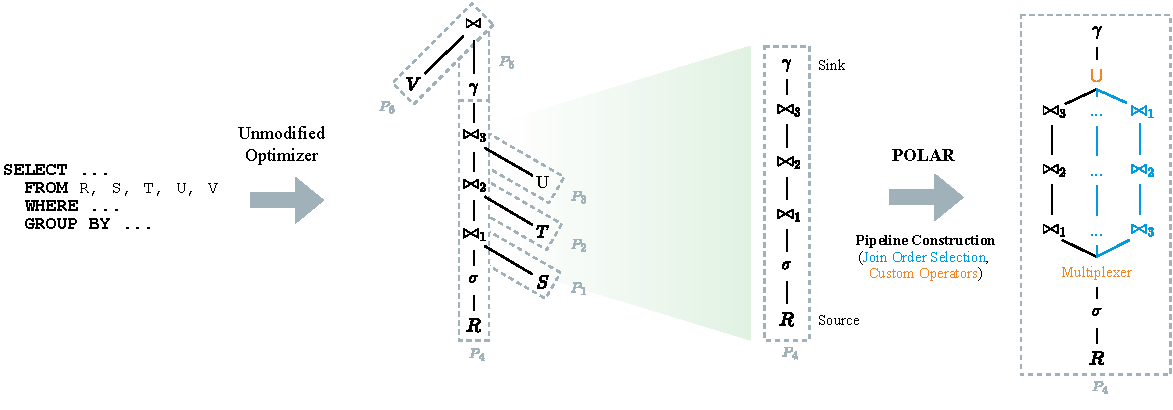
\includegraphics[width=0.82\textwidth]{figures/polar_pipeline-5.pdf}
		\vspace{-0.4cm}
		\caption{POLAR pipeline compilation from input query over standard, pipelined plan to POLAR pipeline.}
    \label{fig:pipeline_design}
		\vspace{-0.12cm}
\end{figure*}

% context
Cost-based query optimizations \cite{SelingerACLP79,moerkotte23} for selecting optimal join orders, join methods, and data access paths are crucial for the end-to-end performance of analytical queries. State-of-the-art exact join ordering algorithms such as DPsize~\cite{SelingerACLP79,HanKLLM08}, DPsub, DPcpp~\cite{MoerkotteN06}, and DPhyp~\cite{MoerkotteN08} rely on dynamic programming for efficient enumeration. These algorithms yield optimal execution plans, but only under the assumption of precise cardinality estimates.

\textbf{Cardinality Estimation Challenges:} Estimating precise cardinalities for intermediate results of complex queries remains a stubbornly difficult problem~\cite{LeisGMBK015}. First, most systems assume uniform distributions (no skew) and independence of predicates (no correlation) \cite{IlyasMHBA04}. These simplifying assumptions often cause under-estimation, which is problematic due to plan choices with poor asymptotic behavior~(\eg nested-loop joins), which perform poorly for larger intermediates \cite{IlyasMHBA04,LeisGMBK015}. Second, too coarse-grained statistics (\eg histograms \cite{KanneM10} or sketches \cite{IzenovDRS21}) may misrepresent clustered data. Third, user-defined functions and new environments (\eg federated, raw data) often do not allow obtaining statistics \cite{HueskePSRBKT12,JosifovskiSHL02,ReyFN23}. Fourth, complex queries with many operators are difficult to estimate because errors propagate exponentially \cite{IzenovDRS21,IoannidisC91,MoerkotteNS09}. Although recent work on ML-based estimators \cite{KipfKRLBK19,DuttWNKNC19,YangLKWDCAHKS19}, learning to distrust certain estimates \cite{MarcusNMZAKPT19}, and learning to rank plans \cite{BehrMK23} offer benefits, they do not solve all problems above.

\textbf{Adaptive Query Processing (AQP):} In the past two decades, a spectrum of AQP techniques \cite{BabuB05,DeshpandeIR07,IvesDR07,DeshpandeHR06} has been devised to address the challenges of unknown and changing data characteristics. Many AQP techniques follow the classical MAPE control loop of monitoring, analyzing, planning, and executing \cite{IvesDR07,mape05,AboulnagaHLLMPR04}. Existing techniques include inter-query optimization with learned cardinalities for expressions \cite{BrunoC02,ChenR94,StillgerLMK01}, late binding with re-optimization at pipeline breakers \cite{DeshpandeHR06} or parameter binding \cite{BizarroBD09}, inter-operator re-optimization at checkpoints \cite{KabraD98}, progressive and pro-active re-optimization with validity ranges \cite{MarklRSLP04,BabuBD05}, intra-operator adaptivity with union stitch-up plans \cite{IvesHW04}, intra-query adaptivity via reinforcement learning \cite{TrummerWMMJA19,TrummerWWMMJAR21,WeiT22}, as well as tuple routing policies in Eddies \cite{HellersteinA00,Arpaci-Dusseau03,Deshpande04,BizarroBDW05}. Many of these strategies require both optimizer and runtime extensions for effective and efficient adaptivity.

\textbf{Robust Query Processing:} An alternative mitigation strategy for poor cardinality estimates is robust query processing \cite{Haritsa20}. The influential Picasso project \cite{Haritsa10} on plan diagrams \cite{ReddyH05} revealed that state-of-the-art DBMS compile many very specialized plans that are only optimal in a small subspace of cardinalities. Since these cardinalities are difficult to estimate, robust query processing seeks to find a small number of plans that together cover a broad range of cardinalities \cite{DDH07,DDH08}. Despite a sequence of valuable improvements \cite{DDH08,AbhiramaBDSH10,GraefeGKP12,DuttH14} (including so-called plan bouquets \cite{DuttH14}), many of these strategies are offline approaches and largely intractable for intra-query or intra-operator adaptation during runtime \cite{Haritsa20}. 

\textbf{POLAR Overview:} Although AQP comprises many valuable ideas, only very few are implemented by data(base) systems in practice. We attribute this largely to the induced complexity of intertwining planning and execution, difficulties in testing and debugging, and potential performance regressions due to overheads of adaptivity. Inspired by tuple-routing and self-scheduling (queue-based) systems, we introduce POLAR as a novel adaptive processing approach of join pipelines. We enhance left-deep join pipelines with alternative join orders during planning, perform regret-bounded tuple routing for exploration, and process most data through \emph{plans of least resistance} (i.e., plans with few intermediates). In contrast to tuple routing in Eddies and SkinnerDB, POLAR is non-invasive to the optimizer and runtime, has low and bounded overhead, and does not require state management (e.g., partially-built hash tables).

\textbf{Contributions:} Our primary contribution is the concept of plans of least resistance (POLAR) as a new AQP technique designed for simple system integration and bounded overhead. Our detailed contributions include the novel POLAR design and its evaluation:
\begin{itemize}
    \item \emph{Pipeline Design:} We introduce a holistic, non-invasive pipe\-line design from objectives over pipeline compilation and join order selection to parallel pipeline processing with performance tracking (Section~\ref{pipeline-design}).
    \item \emph{Routing Strategies:} We propose an extensible multiplexer operator and several routing strategies, as well as describe their trade-offs and runtime characteristics (Section~\ref{sec:routing_strategies}).
		\item \emph{SSB-skew Benchmark:} As a basis for evaluating AQP systems on data with correlations and clustering, we introduce and share the new SSB-skew benchmark (\href{https://github.com/d-justen/duckdb-polr/tree/master/benchmark/ssb-skew}{SSB-skew repository}).
    \item \emph{Experiments:} Using a variety of benchmarks (JOB, SSB, SSB-skew), we systematically study the performance characteristics of a POLAR prototype in DuckDB~\cite{RaasveldtM19}. We evaluate different join order selection and routing strategies and compare with different AQP systems (Section~\ref{experiments}).
\end{itemize}


%% THE PLAN OF LEAST RESISTANCE
%%%%%%%%%%%%%%%%%%%%%%%%%%%%%%%%%%%%%%%%%%%%%%%%%%%%%%%%%%%%%%%%%%%%%%%%%%%%%%%%%%%%
%% PIPELINE DESIGN
%%%%%%%%%%%%%%%%%%%%%%%%%%%%%%%%%%%%%%%%%%%%%%%%%%%%%%%%%%%%%%%%%%%%%%%%%%%%%%%%%%%%

\begin{table}[!b]
	\centering
	\caption{System Integration and Bounded Overhead.}
	\vspace{-0.31cm} 
    \setlength\tabcolsep{6.62pt}
	\begin{tabular}{l|cc|c}
	  \toprule
		\textbf{Approach} & \textbf{Separation} & \textbf{Reuse} & \textbf{Bounded Overhead} \\
		\midrule
        Eddies    & $\times$ & $\times$ & $\times$ \\
		SkinnerDB & $\times$ & $\times$ & \checkmark \\
        LIP       & (\checkmark) & \checkmark & $\times$ \\
        \midrule
        POLAR     & \checkmark & \checkmark & (\checkmark) \\
		\bottomrule
	\end{tabular}
    %\vspace{-0.1cm}
	\label{tab:comparison}
\end{table}

\section{Pipeline Design}
\label{pipeline-design}
%
% pipeline enhancement, telemetry, parallelism
POLAR is an adaptive join processing approach designed for non-invasive integration into common database systems with support for vectorization and operator pipelining. In contrast to other AQP techniques, POLAR pipelines do not require fine-grained intertwining of existing optimizers and runtime systems. As shown in Figure~\ref{fig:pipeline_design} (right), we enhance amenable pipelines with additional join orders. At runtime, we measure the performance of these orders and route tuples to well-performing orders while exploring others using a regret budget. This section introduces POLAR's design objectives and gives an overview of the compilation and execution of POLAR pipelines and related essential primitives.

\subsection{Design Objectives}
\label{sec:objectives}

We largely attribute the stagnant adoption of adaptive join processing approaches to difficult system integration and problematic performance regressions. Accordingly, we propose a non-invasive approach specifically designed for low and bounded overhead. In the following, we define these objectives and distinguish POLAR from existing AQP systems along these dimensions (in Table \ref{tab:comparison}). As bitmap filtering is increasingly adopted in popular database systems~\cite{DingCN20, LeeDNC23}, we also compare POLAR to Lookahead Information Passing~\cite{ZhuPSP17} (LIP) as a representative candidate. 

\textbf{Non-invasive System Integration:} We call an AQP system non-invasive if it clearly separates compilation from execution (no plan generation at runtime) because this separation simplifies debugging and testing. Furthermore, for simple system integration and maintenance, a non-invasive AQP system should reuse existing infrastructure such as the query optimizer and physical operators. Eddies~\cite{HellersteinA00} and SkinnerDB~\cite{TrummerWMMJA19} intertwine query processing phases, and require specific optimizers and operators. LIP mostly adheres to non-invasiveness but generates new bloom filter orders at runtime.

\textbf{Bounded Overhead:} Preventing major performance regressions on any workload---even if adaptation is not beneficial---is essential for enabling AQP by default. Accordingly, an AQP system should provide bounds for the overhead of adaptivity (e.g., exploration of alternative join orders). Eddies and LIP do not define bounds for their overheads, SkinnerDB gives a strict bound based on the single best (robust) join plan, and POLAR provides a probabilistic bound on the number of intermediates incurred for exploration.

\vspace{-0.1cm}
\subsection{POLAR Pipeline Compilation}
\label{pipeline-enhancement}

%overview 
During query compilation (cf. Figure~\ref{fig:pipeline_design}), we replace amenable operator pipelines with POLAR pipelines. A POLAR pipeline contains alternative join orders and two dedicated operators: a \textit{multiplexer} (for tuple routing) and an \textit{adaptive union} $\cup$ (for result consolidation). In the following, we describe the pipeline selection, the dedicated operators, and the pipeline transformation in more detail.

\textbf{Pipeline Construction:} After query optimization and generation of a query execution plan---consisting of multiple operator pipelines---POLAR replaces all pipelines of left-deep join trees with at least two joins (where the right-hand-sides are build sides, and left-hand-side intermediates are probed in a pipelined fashion). The pipeline's source is the left-most node and fixed as POLAR's source of input tuples for the tuple routing. Our approach generates a set of alternative join orders using a \emph{join order selection} algorithm (cf. Section~\ref{sec:paths}) and includes them with the original join order. Although focusing only on existing join pipelines is limiting, it allows for a system integration without changing the query optimizer and robust performance that is at least as good as the original plan. If the original plan contains pipelines with multiple joins, POLAR can improve these pipelines via alternative orders.

\textbf{Custom Operators:} Additionally, we introduce two new operators into each POLAR pipeline for tuple routing. The \emph{multiplexer} (cf. Section \ref{sec:routing_strategies}) accepts bags of tuples from the source table and determines the next path and the number of tuples to route to that path. It uses performance indicators from previous path runs to make routing decisions. After each path run, a lightweight \emph{adaptive union} operator processes the results from the last join. Besides normal union-all semantics, this operator re-arranges the additional columns from the joins to a consistent order of the original plan.

\textbf{Pipeline Transformation:} Finally, we replace the existing operator pipeline with a POLAR pipeline consisting of the multiplexer, the set of join orders, and the adaptive union. The individual join orders reuse the read-only hash tables of the build sides without redundant allocation. This transformation does not break the pipeline to prevent further materialization and multiplexing. Other non-blocking operators (\eg projections, filters) and the pipeline sink (\eg aggregation) also remain unchanged. The POLAR pipeline allocates space for state per alternative join order (e.g., operator caches, intermediate result vectors). Thus, the space overhead grows linearly with the number of join orders but is negligible in practice.

\vspace{-0.1cm}
\subsection{Join Order Selection}
\label{sec:paths}

When generating alternative join orders for individual pipelines, we aim to compose a diverse set of orders that could handle a wide range of mis-estimated cardinalities and clustered data. The selection strategy should find good plans early (\ie be robust for large pipelines), should not re-invoke the query optimizer (\ie ensure non-invasive integration and low overhead), and should pick few complementary join orders (\ie reduce the amount of exploration overhead). To this end, we propose two novel, anytime join order selection strategies that do not require optimizer invocations, as well as additional heuristics to serve as baselines.

\begin{algorithm}[!t] \small
\caption{Selectivity Space Sampling}\label{alg:enumeration1}
\begin{algorithmic}[1]
\Require{Joins $J$, Max Join Orders $\mathit{MAX}$, Max Iterations $\mathit{maxi}$}
\Ensure{Join Orders $T$}
\State $T \gets \emptyset$, $i \gets 0$
\State $\mat{D} \gets \textsc{discretizeSelectivities}(J)$ \Comment{exponential decay}
\While{$\card{T} < \mathit{MAX} \wedge i < maxi$} 
  \State $d_i \gets \textsc{sample}($\mat{D}$)$, $i \gets i+1$ \Comment{$\card{J}$ selectivities} 
	\State $T \gets T \cup \textsc{DPSize}($J$, d_i)$ \Comment{keep distinct optimal join orders}
\EndWhile
\State \Return $T$
\end{algorithmic}
\end{algorithm}

\begin{algorithm}[!t] \small
\caption{Next-best Join Order Search}\label{alg:enumeration2}
\begin{algorithmic}[1]
\Require{Joins $J$, Edge Counts $n_0, ..., n_{\card{J}} \in N$, Max Join Orders $\mathit{MAX}$}
\Ensure{Join Orders $T$}
\State $R \gets \emptyset$
\State $S \gets \textsc{LegalJoinCandidates}(R, J)$ \Comment{Find first join candidates}
\For{$i \gets 0$ \textbf{to} $n_0$}
    \Comment{Consider $n_0$ of the candidates}
    \State $s_i \gets \textsc{GetNextJoin}(S)$
    \State $\mathit{prio} \gets (\card{R}, i)$
    \State $pqueue.\textsc{Enqueue}(prio, R, s_i)$
    \State $S \gets S \setminus s_i$
\EndFor
\While{$!pqueue.\textsc{Empty}()$ and $\card{J} < \mathit{MAX}$}
    \State $R, s \gets pqueue.\textsc{Dequeue}()$ \Comment{Remove next item}
    \State $R \gets R \oplus s$
    \If{$\card{R} = \card{J} - 1$}
        \State $R \gets R \oplus J \setminus R$ \Comment{Append remaining join}
        \State $T \gets T \cup R$
    \Else
        \State $S \gets \textsc{LegalJoinCandidates}(R, J)$
        \For{$i \gets 0$ \textbf{to} $n_{\card{R}}$}
            \State $s_i \gets \textsc{GetNextJoin}(S)$
            \State $\mathit{prio} \gets (\card{R}, i)$
            \State $pqueue.\textsc{Enqueue}(prio, R, s_i)$
            \State $S \gets S \setminus s_i$
        \EndFor
    \EndIf
\EndWhile
\State \Return $T \cup \textsc{GetOriginalJoinOrder}()$
\end{algorithmic}
\end{algorithm}

\textbf{S1 \textsc{SelSampling}:} For good coverage of complementary join orders, we propose selectivity-space sampling in Algorithm~\ref{alg:enumeration1}, a method to sample the space of unknown selectivities and generate optimal join orders for each sample. Inspired by progressive parametric query optimization \cite{BizarroBD09}, the discretized selectivities of base table predicates and joins form a d-dimensional grid, which we sample uniformly. For each sampled point, we then call DPsize with $C_{out}$ cost model to generate the optimal plan for this scenario. In order to efficiently explore alternative orders, we use an exponential discretization (e.g., 0.1, 0.01, 0.001). For predicates and foreign key/primary key joins, we multiply this selectivity with $\card{R}$; for general joins with $\card{R \times S}$. Compared to brute-force creation of all left-deep join orders ($2^{n-1}$ for chain, $n!$ for clique queries) \cite{moerkotte23}, \textsc{SelSampling} generates only up to $\mathit{MAX}$ join orders, and can be terminated anytime (e.g., if $\mathit{maxi}$ samples were taken).

\textbf{S2 \textsc{NextBestSearch}:} With Algorithm~\ref{alg:enumeration2}, we introduce an alternative join order selection approach called \emph{next-best search} that uses a priority queue to explore join candidates in a breadth-first search manner. The algorithm considers the search space a tree with parent-child sequences representing join orders. In this tree, the set of all paths from root to leaf node is the set of all legal join orders. Figure~\ref{fig:search_space} shows an example of such a join order search tree. We explore the tree by retrieving all possible join candidates $S$ for a given node $R$. The function $\textsc{GetNextJoin(S)}$ then determines the $n_{\card{R}}$ fittest candidates, with $n_{\card{R}}$ being the number of edges to consider at a certain tree level. For each candidate $s_i$, the algorithm pushes an item containing the current node, the join candidate $s_i$, the tree level (\ie the length of the current join sequence $R$), and the fitness index $i$. The priority queue compares its items based on the tree level and fitness index---similar to recent heuristic search strategies in join enumeration to maximize pruning \cite{HaffnerD23}---so that the fittest join candidate in the lowest level is always the next item to process. Depending on the values for $N=(n_0, \ldots, n_{\card{J}})$, the maximum number of join orders $\textit{MAX}$, and $\textsc{GetNextJoin}$, the algorithm allows finding different join order subsets. For example, setting $N$ to increasing values favors diversity of join candidates for the rear joins of a join order. We utilize two versions of $\textsc{GetNextJoin}$:
\begin{itemize}
\item \textbf{S2a \textsc{GetRandom}:} Pick a random join candidate.
\item \textbf{S2b \textsc{GetMinCard}:} Pick the join candidate with the lowest estimated cardinality.
\end{itemize}

\begin{figure}[!t]
    \vspace{-0.1cm}
    \centering
    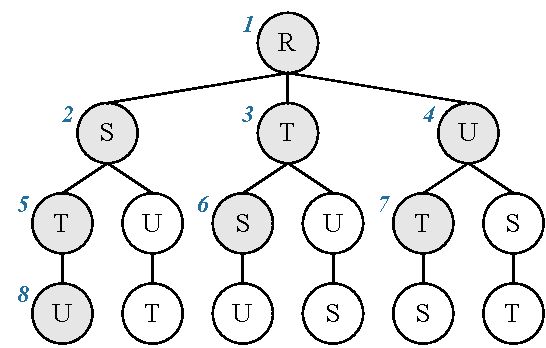
\includegraphics[width=0.5\linewidth]{figures/join_order_search_space-3.pdf}
    \vspace{-0.15cm}
    \caption{The Join Order Search Space as a Tree: A path from root to leaf denotes a sequence of joins. The visited nodes are marked in gray, and the digits indicate the order in which they are visited using the Next-Best Join Order Search. At step 8, the algorithm emits the first join order $\langle R, S, T, U \rangle$.}
    \label{fig:search_space}
    \vspace{-0.35cm}
\end{figure}

\textbf{Basic Heuristics:} Besides the search-based approaches, we use two simple additional heuristics to generate alternative join orders: 
\begin{itemize}
\item \textbf{S3 \textsc{PushDown}:} Permute the original join order such that each join gets pushed to be the first in the join order once if legal (assuming that the first join in the pipeline often has the largest performance impact~\cite{DBLP:conf/damon/SchubertGZM23}).
\item \textbf{S4 \textsc{PullUp}:} Pull each join to the last position in the join order if possible (assuming that join blowups may be mitigated if the problematic join is pulled up to the end of the join order as other joins may filter its input).
\end{itemize}

\subsection{Pipeline Execution}\label{sec:execution}

During query execution, POLAR routes tuples from the source table of a pipeline through multiple join paths. The pipeline executor of these paths reports the performance and calculates their \emph{resistance} for future routing decisions. By using thread-local state (e.g., for tuple buffers and multiplexer state), POLAR can execute its pipelines in parallel without blocking. In this section, we discuss the related techniques for pipeline orchestration, our resistance metric, and parallel execution strategies in detail.

\textbf{Pipeline Orchestration:} To process a POLAR pipeline, the database system spawns a custom POLAR pipeline executor responsible for passing tuples to the operators according to the multiplexer's routing decisions. 
The executor fetches chunks (\ie mini-batches or sets of tuples) from the source and passes them sequentially through the pipeline. The multiplexer consumes a chunk and returns an output chunk containing a subset of the input (or the whole input) and the index of the next join order to pass the subset to. If the multiplexer does not return all tuples from the input, the executor re-invokes the multiplexer with the same input chunk in the next iteration to emit the next tuple subset instead of fetching a new chunk from the source. After routing the chunk to its dedicated join order, the executor passes the chunk to the adaptive union, other pipeline operators, and finally the pipeline sink. During this process, the executor counts the number of intermediates appearing within the path as a performance indicator. We chose intermediates over time because they allow isolated observations (irrespective of other operators and parallelism), and the related $C_{out}$ cost model is known to be simple yet accurate \cite{moerkotte23, LeisGMBK015}. After fully processing one multiplexer output chunk in a join order, the executor reports back the number of intermediates from that routing iteration to the multiplexer. This design allows adapting the \emph{plans of least resistance} to clustered data. For example, table $R$ from Figure~\ref{fig:pipeline_design} may have many matches with $S$ and few with $T$ for its first half of rows but behave the opposite for its second half. For this reason, POLAR never discards previously generated join orders.

\begin{figure}[!b]
    \centering
		\vspace{-0.35cm}
    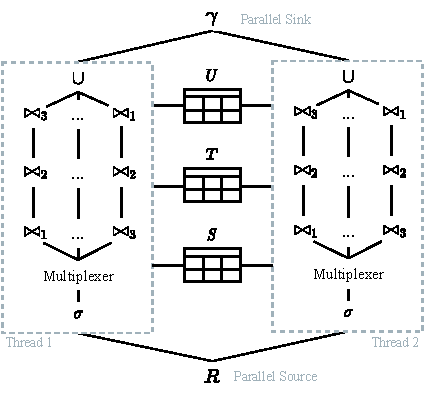
\includegraphics[width=0.82\linewidth]{figures/parallel-exec-2-2.pdf}
    \vspace{-0.5cm}
    \caption{Parallel Execution: Each thread processes a pipeline with an isolated state, sharing build sides to probe into.}
    \vspace{-0.25cm}
    \label{fig:parallel-exec}
\end{figure}

\textbf{Resistance Metric:} As a proxy for performance, the POLAR executor calculates a join order \emph{resistance}. This quantity comprises the sum of intermediate results $I$ observed in the current routing iteration, the number of tuples routed to the current join order $T$, and a constant $w$ representing the overhead of a routing iteration without intermediate results. We calculate the resistance as ${r = \frac{I}{T} + w}$. The constant $w$ prevents edge cases of a routing iteration with zero intermediates counting as infinitely better than an iteration with few intermediates. If only a few tuples are routed to a join order, the resistance may not be representative for a larger set of tuples. Consequently, the executor applies a moving average from previous iterations for smoothing fluctuations.

\textbf{Parallel Execution:} Similar to traditional data-parallel processing, POLAR executes pipelines in a multi-threaded fashion using multiple executors with thread-local states (cf. Figure~\ref{fig:parallel-exec}). The executors concurrently fetch batches of tuples from the source and push results to the sink. Each executor has an isolated multiplexer state and calculates the path resistances solely based on its fetched tuples. Note that the executors only isolate their processing states but share build-side data structures such as read-only hash tables. With the input tuples, the executor follows the paths sequentially and independently from each other. The lack of global multiplexing may delay finding better paths because each multiplexer computes resistances individually. However, this parallelization strategy avoids synchronization among the executors and ensures correct resistance metrics for clustered data. As an alternative baseline parallelization strategy, POLAR also supports spawning one thread per join order and applying a backpressure mechanism to route tuples in a self-scheduling manner (cf. Section~\ref{sec:backpressure}).


%%%%%%%%%%%%%%%%%%%%%%%%%%%%%%%%%%%%%%%%%%%%%%%%%%%%%%%%%%%%%%%%%%%%%%%%%%%%%%%%%%%%
%% ROUTING STRATEGY
%%%%%%%%%%%%%%%%%%%%%%%%%%%%%%%%%%%%%%%%%%%%%%%%%%%%%%%%%%%%%%%%%%%%%%%%%%%%%%%%%%%%


\section{Routing Strategies}
\label{sec:routing_strategies}

At the core of POLAR pipeline execution is the multiplexer operator that makes routing decisions for exploration and exploitation to determine the number of input tuples for each join order. To this end, the pipeline executor passes an input chunk to the multiplexer, which uses a \emph{routing strategy} to return the next join path index and a subset of the tuples to route. The routing strategies attempt to follow the \emph{plans of least resistance}, which is the---potentially temporally changing---sequence of join order paths that incur the fewest number of intermediates. In this section, we first discuss the overall multiplexer algorithm, followed by four dedicated routing strategies used by the multiplexer and one self-scheduling strategy.

%%%%%%%
\subsection{Overall Multiplexer Algorithm}
\label{sec:multiplexer}

Algorithm \ref{alg:multiplexer} shows the overall multiplexer algorithm. In the initialization phase, the multiplexer sends a small number of tuples to each join order with a resistance of zero (\ie an uninitialized join order without reported resistance) to measure initial performance. When all join orders are initialized, the multiplexer requests a tuple distribution from a configurable routing strategy. The distribution indicates the fraction that each join order receives from the current input chunk. The algorithm finally returns the join order index with the largest fraction and its respective input tuple count. If the multiplexer does not emit all tuples from the input chunk, the multiplexer emits the remaining tuples from the tuple distribution in the next iteration until the input chunk is fully processed (cf. Section~\ref{sec:execution}).
%
In the following, we introduce four different routing strategies implementing the tuple distribution method. Assuming that POLAR is executed in a vectorized database system, the implementation must trade-off path optimality (following the cheapest path through the join orders) and operator cache friendliness (minimizing the number of join order switches). The caching aspect can impact the processing performance as the pipeline executor must flush all operator caches buffering intermediates for vectorization before reporting the join order resistance to ensure that each input tuple has been fully processed and was thus correctly counted. Additionally, processing without buffering or too frequent plan switches may increase the number of instruction cache misses~\cite{SirinTPA16}. 

\begin{algorithm}[!t]
\caption{Multiplexer}\label{alg:multiplexer} \small
\begin{algorithmic}[1]
\Require{Tuple Distribution $T$, Resistances $\mat{W}$} 
\Ensure{Join Order Index $\mathit{idx}$, Tuple count $c$}
\If{$\exists t_{\mathit{idx}} \in T: t_{\mathit{idx}} > 0$}
    \State $\mathit{fraction} \gets t_{\mathit{idx}}$ \Comment{Route tuples from previous multiplexing}
    \State $t_{\mathit{idx}} \gets 0$
    \State\Return $\mathit{idx}$, $\mathit{fraction} \cdot \mathit{INPUT\_SIZE}$
\ElsIf{$\exists w_{\mathit{idx}} \in \mat{W}: w = 0$} \Comment{Initialize join order}
    \State\Return $\mathit{idx}$, $\textsc{INIT\_COUNT}$
\EndIf
\State $T \gets \textsc{GetTupleDistribution}(\mat{W})$
\State $\mathit{idx}, \mathit{fraction} \gets \textsc{max}(T)$
\State $t_{\mathit{idx}} \gets 0$
\State\Return $\mathit{idx}$, $\mathit{fraction} \cdot \textsc{INPUT\_SIZE}$
\end{algorithmic}
\end{algorithm}

%%%%%%%
\subsection{Static Selection}

Static routing strategies, or path selection approaches, do not perform any exploration apart from initialization. For this reason, they are very simple to implement, and thus, we omit their pseudo-code of $\textsc{GetTupleDistribution}$ but provide high-level descriptions.

\textbf{R1 \textsc{InitOnce}:} This simple strategy retrieves the join order with the lowest resistance after the initialization phase and then routes every following chunk to that join order. \textsc{InitOnce} is extremely cache-friendly (i.e., in terms of tuple buffering in operator pipelines) because it does not require path switching or counting intermediates throughout the query. However, this strategy is prone to bad routing if a join order only performs well for the first few tuples. Moreover, it is unable to find well-performing paths if different join orders are optimal for different data clusters of the source.

\textbf{R2 \textsc{Opportunistic}:} The \textsc{Opportunistic} routing strategy is similar to \textsc{InitOnce} but makes use of the resistance reports after routing each chunk. If the reported resistance of the current join order exceeds the resistance of another, it routes the next input chunks to that join order. This approach allows switching join orders if the previous order deteriorates. However, the decision is solely based on the resistance of a single join order and old initialization results of others, which may miss additional opportunities, such as better plans for clusters of data. Cache flushing is needed but can be reduced by only updating the resistance after every $n$-th chunk, trading granularity with cache-efficiency.  

%%%%%%%
\subsection{Pro-active Exploration}

\begin{figure*}[!t]
    \centering
    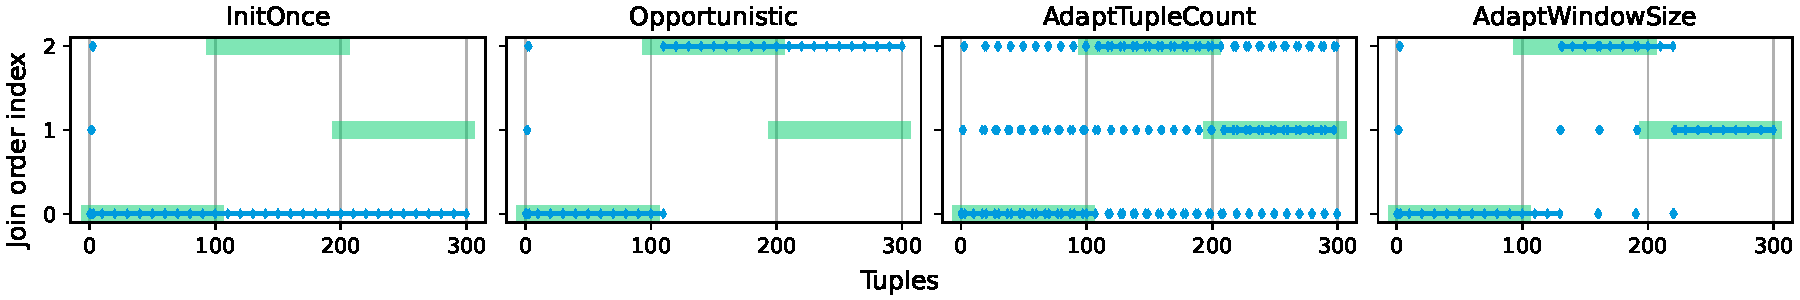
\includegraphics[width=0.99\linewidth]{figures/routing_example.pdf}
		\vspace{-0.2cm}
    \caption{Behavior of four different routing strategies in a single-threaded example scenario with 30 input batches of 10 tuples each (green: optimal join paths, blue diamond: multiplexer invocations, blue line: path chosen by routing strategy).}
    \vspace{-0.1cm}
    \label{fig:routing_example}
\end{figure*}

In order to handle varying data characteristics and find well-per\-form\-ing join orders, routing strategies need to pro-actively explore alternative join orders. To this end, these strategies periodically route tuples to join orders that performed sub-optimal in the past. We introduce two strategies that both use the notion of an \emph{exploration budget} that probabilistically bounds the overhead the strategy allocates for finding the optimal join path (cf. Section~\ref{sec:objectives}). The two following strategies use the exploration budget to calculate a tuple distribution over the join orders, producing additional intermediates based on the resistances measured so far.

\begin{algorithm}[!t] \small
\caption{GetTupleDistribution -- \textsc{AdaptTupleCount}}\label{alg:adapt_tuple_count}
\begin{algorithmic}[1]
\Require{Resistances $\mat{W}$, \textbf{Output:} Tuple Distribution $T$}
%\Ensure{Tuple Distribution $T$}
\State $T \gets \textsc{Initialize}(\card{\mat{W}}, 1)$
\State $\mat{W} \gets \textsc{SortInc}(\mat{W})$
\State $\mathit{cost} \gets \textsc{LastElement}(\mat{W})$
\For{$i \gets \card{\mat{W}} - 1$ \textbf{to} $0$}\Comment{Calculate distribution bottom-up}
    \State $\mathit{target} \gets w_i \cdot (1 + \textsc{BUDGET})$
    \State $\mathit{decrease} \gets \frac{w_i - \mathit{target}}{w_i - \mathit{cost}}$
    \For{$j \gets i+1$ \textbf{to} $\card{\mat{W}}$}\Comment{Adjust fractions to new target}
        \State $t_j \gets t_j \cdot \mathit{decrease}$
    \EndFor
    \State $t_i \gets 1 - \mathit{decrease}$
    \State $\mathit{cost} \gets \mathit{target}$
\EndFor
\State\Return $T$
\end{algorithmic}
\end{algorithm}


\begin{algorithm}[!t] \small
\caption{GetTupleDistribution -- \textsc{AdaptWindowSize}}\label{alg:adapt_window_size}
\begin{algorithmic}[1]
\Require{Resistances $\mat{W}$, \textbf{Output:} Tuple Distribution $T$}
%\Ensure{Tuple Distribution $T$}
\State $T \gets \textsc{Initialize}(\card{\mat{W}}, 0)$
\State $t_{\textsc{minIndex}(W)} \gets 1$ \Comment{Route all tuples to least resistant order}
\State $\mathit{size}$, $\mathit{offset} \gets \textsc{GetWindowState}()$
\If{$\mathit{size} = 0$} \Comment{Determine window size}
    \State $W^{\prime} \gets \mat{W} \setminus \textsc{min}(\mat{W})$
    \State $\mathit{size} \gets \frac{1}{\textsc{INPUT\_SIZE}} \cdot \frac{\sum w^{\prime}_i \cdot \textsc{INIT\_COUNT}}{\textsc{BUDGET} \cdot \textsc{min}(W)}$
\EndIf
\If{$\mathit{offset} < \mathit{size}$}
    \State $\mathit{offset} \gets \mathit{offset} + 1$
\Else \Comment{Re-explore join orders next time}
    \State $\mat{W} \gets \textsc{SetToZero}(\mat{W} \setminus \textsc{min}(\mat{W}))$ \Comment{Reset resistances}
    \State $\mathit{offset}, \mathit{size} \gets 0$
\EndIf
\State $\textsc{SetWindowState}(\mathit{size}, \mathit{offset})$
\State\Return $T$
\end{algorithmic}
\end{algorithm}

\textbf{R3 \textsc{AdaptTupleCount}:} For each input chunk, the \textsc{AdaptTupleCount} strategy determines a tuple distribution that (assuming previous resistances) would stay within the exploration budget relative to the best path's intermediate count.
%
The strategy initializes the output tuple fractions with ones (line 1), orders paths by their resistances (line 2), and adjusts the distribution in a bottom-up fashion. We start by reducing the problem to the two join orders with the highest resistances. The target cost is based on the lower resistance and the exploration budget, which we then use to calculate a \textit{decrease} factor (line 6). By multiplying that factor with the join order's tuple fraction, we find the amount of tuples that must be sent to the worst join order to stay within the exploration budget based on the resistance of the second-last join order. Consequently, the amount for the second-last order is $1 - \mathit{decrease}$ (line 10). We calculate these values for the next-best join order while decreasing the fractions of the orders with higher resistances until we reach the first join order. \textsc{AdaptTupleCount} calculates tuple distributions for each incoming chunk, allowing for fine-grained path exploration bounded by the exploration budget. However, splitting each chunk into smaller sets of tuples obstructs vectorized execution and causes many cache flushes to report resistances. To reduce the number of splits per chunk, the algorithm could serve only join orders receiving more than $n$ tuples, redistributes unserved tuples, and recalls them when calculating the next distribution.

\textbf{R4 \textsc{AdaptWindowSize}:} In contrast to \textsc{AdaptTupleCount}, the \textsc{AdaptWindowSize} strategy does not calculate individual tuple counts per join order. Instead, this strategy either routes complete chunks or a static, low number of tuples and adapts the window size (\ie number of input chunks) within which it will only serve the best join order. When exceeding the window, it re-initializes the remaining join orders by routing a small number of tuples to each of them. The internals of this strategy are shown in Algorithm~\ref{alg:adapt_window_size}, which distinguishes between three cases. Irrespective of the case, this strategy always returns a tuple distribution in which the best order receives the whole input chunk (line 2). If there is no window size calculated yet (line 4), we estimate the number of intermediates occurring in a reinitialization phase based on the resistances and adjust the number of tuples for reinitialization accordingly. We then divide the cost estimate by the overhead allowed by the exploration budget resulting in the number of tuples that should be routed to the best join order before reinitializing the others. The number of tuples per chunk scales this value down to the window size (line 6). If the current offset does not exceed the window size, we increment it (line~9). Finally, if the window size is exceeded, we set the resistances for all join orders, except the best, to zero (line 12) to trigger re-initialization on the next invocation. By routing multiple chunks to the same join order, the \textsc{AdaptWindowSize} strategy better allows for vectorization and can defer cache flushing until the window size is exceeded. On the other hand, its path exploration granularity is more coarse-grained than \textsc{AdaptTupleCount} as changes in resistances may appear within the routing window.

\begin{example2}[Routing Example] To illustrate the behavior of the routing strategies, Figure \ref{fig:routing_example} compares their  decisions in an example scenario (three join orders, 30 input chunks of 10 tuples each). The resistances of the join orders change every 10 chunks, namely $C_0 \gets \langle 1, 10, 15 \rangle$, $C_{10} \gets \langle 10, 15, 5 \rangle$, and $C_{20} \gets \langle 10, 1, 5 \rangle$. The resulting optimal path changes from 1st to 3rd to 2nd (indicated as green solid lines). The blue diamonds show the multiplexer invocations of the different paths, and the blue line indicates the chosen path. \textsc{Init\-Once} tests every join order once and follows the initially optimal path. The \textsc{Opportunistic} strategy switches to the correct path after the first one deteriorates but misses the second switch. \textsc{AdaptTupleCount} correctly adapts to the optimal join paths but requires many switches and multiplexer invocations, including cache flushing. Finally, \textsc{AdaptWindowSize} first uses a large window and thus detects the join order switch only after a delay. Later, it reduces the window size as the difference between the resistances decreases. Hence, the next switch comes after a shorter delay due to window resizing.
\end{example2}

\subsection{Self-scheduling}\label{sec:backpressure}

\textbf{R5 \textsc{Backpressure}:} To enable comparing against a self-scheduling strategy without parameters, we include a \enquote{backpressure} strategy. Instead of using a multiplexer, the POLAR pipeline spawns individual threads for each join order so that each thread concurrently pulls new input chunks. The approach does not depend on a budget and simply favors faster join orders as they can pull more chunks per time unit than others. The \textsc{Backpressure} strategy does not rely on multiplexing, does not require any operator cache flushes, and thus, fully supports vectorized execution. However, with potentially many join orders, this strategy has the intrinsic limitation that the majority of threads waste CPU cycles on sub-optimal paths.

%%%%%%%%%%%%%%%%%%%%%%%%%%%%%%%%%%%%%%%%%%%%%%%%%%%%%%%%%%%%%%%%%%%%%%%%%%%%%%%%%%%%
%% LIMITATIONS
%%%%%%%%%%%%%%%%%%%%%%%%%%%%%%%%%%%%%%%%%%%%%%%%%%%%%%%%%%%%%%%%%%%%%%%%%%%%%%%%%%%%

\section{Limitations and Scope}
\label{sec:limits}
%
POLAR is designed for adaptive query processing with non-invasive system integration as well as small and bounded overhead. This design leads to certain limitations as its applicability is ultimately dependent on the system's existing query optimizer. 
\begin{itemize}
\item \emph{Amenable Pipelines:} POLAR only replaces left-deep-trees. If the optimizer emits a right-deep tree (where intermediates feed into the build side of hash joins), POLAR cannot generate alternative join orders, as there are no pipelines with more than one join. Support for directed acyclic graphs (DAGs) and bushy trees is interesting future work.
\item \emph{Source Table:} As POLAR replaces normal operator pipelines that consume tuples from a specific source, it cannot change the source (sometimes called driver \cite{LiSMBCL07}) table.
\item \emph{Operator Types:} POLAR only supports pipelines with join sequences. Extended support for additional operators---such as projection, selection, and groupjoin \cite{MoerkotteN11}---is interesting future work as well.
\end{itemize}
%
POLAR is currently most applicable to star-schema workloads with cardinality estimation challenges (\eg parameterized queries, UDFs, correlated data). If the source table contains clustered data (\eg orders sorted by date with different join cardinalities over time), POLAR can further exploit different plans for different data.

%% EXPERIMENTS
\section{Experiments}
\label{experiments}

Our experimental evaluation of a prototype implementation of POLAR studies its general applicability and performance characteristics with a variety of benchmarks. After describing the prototype and experimental setting, we use various micro benchmarks to evaluate the behavior of different strategies and parameters and conduct end-to-end performance comparisons with DuckDB~\cite{RaasveldtM19}, Postgres~\cite{DBLP:conf/sigmod/StonebrakerR86}, SkinnerDB~\cite{TrummerWMMJA19, TrummerWWMMJAR21}, SkinnerMT~\cite{WeiT22}, and Lookahead Information Passing~\cite{ZhuPSP17} in DuckDB. Our major findings are that: 
\begin{enumerate}
\item Non-invasive AQP yields robust end-to-end performance,
\item Offers substantial speedups for certain queries, especially on skewed benchmarks, and
\item Is already effective with small exploration budgets of $\leq$1\,\%. 
\end{enumerate}

\subsection{Experimental Setup}

\textbf{Prototype:} We implemented POLAR in DuckDB, a state-of-the-art OLAP DBMS. The prototype\footnote{We share our prototype and artifacts at \url{https://github.com/damslab/reproducibility}.}, including the different routing and selection strategies, is ~2500 LoC and requires minimal changes to the existing DuckDB code. The input to POLAR is a query plan produced by the DuckDB optimizer, which uses equivalence sets to estimate cardinalities~\cite{thesis/Ebergen22} and DPhyp~\cite{MoerkotteN08} for join ordering.  

\textbf{Evaluation System:} We conducted all experiments on a Lenovo ThinkSystem SR635 server with a single AMD EPYC 7443P CPU at $2.85$\,GHz (24 physical/48 virtual cores), 256\,GB DDR4 RAM at 3.2\,GHz, $1\times 480\,\text{GB}$ SATA SSD, $8\times 2\,\text{TB}$ SATA HDDs (data) and Mellanox ConnectX-6 HDR/200\,Gb Infiniband. We compiled the source code with clang-12 on Ubuntu 20.04.1.

\textbf{Benchmarks:} We evaluate POLAR on the Join Order Benchmark (JOB)~\cite{JoinOrderBenchmark}, Star Schema Benchmark (SSB)~\cite{SSB-ONeil2009-qs}, and a modified SSB with correlation and skew (SSB-skew), both with a scale factor of 100.
%
We introduce SSB-skew as a benchmark with SSB's applicability (long join pipelines, cf. Section~\ref{sec:potential-analysis}) but real-world data characteristics such as cross-correlations, skew, and clustered data. In SSB-skew, most customers are from the US and most suppliers are from Asia. Moreover, the \texttt{part} table references are skewed, so many lineitems belong to a few part categories and brands. The \texttt{lineorder} table is clustered by order date, with a recession of few orders in 1997 and a year of growth in 1998. Finally, the number of lineitems from suppliers in the United States increases over time. SSB-skew uses SSB's original queries except query set 1 (only one join).
%
We do not use TPC-H \cite{tpch} and JCC-H \cite{JCC-H} because (1) their optimal join orders are well-known and often tuned for, and (2) the join orders generated by DuckDB are mostly right-deep trees, not amenable to POLAR. We also considered the LDBC Social Network BI Workload~\cite{LDBC}, but LDBC requires advanced SQL features which are not supported by all systems we compare, and the DuckDB optimizer often generates pipelines with alternating joins and projections, which our prototype does not yet support (cf. Section~\ref{sec:limits}).
%

%%%%%%%%%%%%%%%%%%%%%%%
\subsection{Applicability Study}
\label{sec:potential-analysis}

\begin{table}[!t]
	\centering 
	\caption{Intermediate Tuple Reduction and Coverage of Amenable Piplines -- Total number of intermediate tuples and fraction of total execution time spent in amenable pipelines.}
	\vspace{-0.3cm} \setlength\tabcolsep{5pt}
	\begin{tabular}{lrrrr}
		\toprule
		\textbf{Benchmark} & \textbf{DuckDB} & \textbf{Routing} & \textbf{Static} & \textbf{Coverage}\\
		\midrule
		JOB &     107.49 M &      16.92 M &      25.84 M & 37 \%\\
		SSB &      86.65 M &      55.06 M &      57.83 M & 68 \%\\
		SSB-skew &     929.87 M &      25.15 M &     688.90 M & 97 \%\\
		\bottomrule
	\end{tabular}
	\label{tab:1_2_potential_savings}
\end{table}


In a first series of experiments, we aim to analyze the potential of POLAR by estimating the possible reduction in the number of intermediates with optimal routing strategies. These results serve as a baseline---in terms of an upper bound---for later experiments evaluating the quality of POLAR routing strategies. Furthermore, we also examine the time spent in amenable pipelines. Combining these measures allows estimating the overall potential.

\textbf{Potential Reduction of Intermediates:} Table~\ref{tab:1_2_potential_savings} shows the potential performance improvements achievable with adaptive join order switching. We calculated the potential improvement by measuring the number of intermediate results for all amenable pipelines using DuckDB's default join order, the best static join order for each pipeline, and an estimated optimal routing strategy. We determined this optimal value using a multiplexer debugging mode, routing each input chunk to every legal join order and measuring the minimal number of intermediates.
%
Table~\ref{tab:1_2_potential_savings} shows that dynamic tuple routing reduces the number of intermediates for all benchmarks but the potential improvement over an ideal static join order is most significant with skewed datasets. For JOB, the best static join order produces 25.84\,M tuples compared to 107.49\,M tuples from DuckDB's default join order. Dynamic routing further improves this number to 16.92\,M tuples. This result shows that a better static join order could improve JOB to a large extent without dynamic join order switching at runtime. For SSB, neither join order switching nor better join orders considerably improve the number of intermediates. The best static join order produces 578.23\,M tuples, a moderate improvement over the 747.67\,M tuples in the default DuckDB plan, and dynamic routing yields only a slight additional improvement to 547.40\,M tuples. DuckDB's near-optimal plan for SSB is expected because the benchmark contains well-behaved FK/PK joins and uniform, non-skewed data.
%
For SSB-skew, which includes correlation and skew, the potential for improvement is much higher. The default DuckDB join order produces 2690.05\,M tuples, while the best static join order produces 474.28\,M tuples. Tuple routing further decreases the optimal number of intermediates to 342.67\,M. Thus, SSB-skew benefits from routing about the same as JOB.

\begin{figure}[!t]
    \centering
    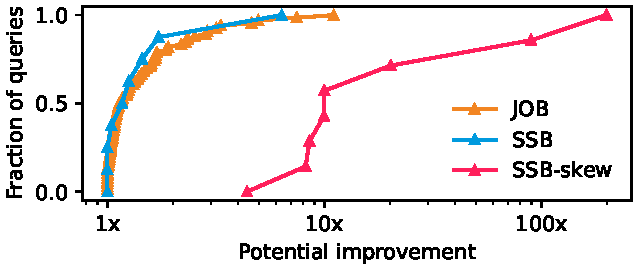
\includegraphics[width=0.95\linewidth]{figures/1_3_potential_query_improvements.pdf}
    \vspace{-0.4cm}
		\caption{Potential Query Performance Improvement.}
    \label{fig:1_3_potential_query_improvements}
		\vspace{-0.5cm}
\end{figure}

\textbf{Coverage of Amenable Pipelines:} Given DuckDB's default query plans, we measure each benchmark's total execution time and the time spent processing POLAR-amenable pipelines (\ie pipelines containing left-deep trees of two or more joins). Comparing the difference of these values yields the \textit{Coverage}, that is, the fraction of time spent in improvable pipelines. Note that the coverage also includes other operators from these pipelines, such as scans and aggregations, which POLAR cannot improve. The Coverage column in Table \ref{tab:1_2_potential_savings} shows that for JOB, DuckDB only spends 36\,\% of the processing time in POLAR-applicable pipelines. Consequently, almost two-thirds of the total execution time cannot be improved by POLAR. For SSB, DuckDB spends 73\,\% of the time in applicable pipelines, but many of them are dominated by large table scans and the joins only account for a small portion of the time. For SSB-skew, DuckDB spends almost all of the execution time (99\,\%) in applicable pipelines, and joins account for a large fraction of that time, providing substantial room for performance improvements.

\textbf{Potential Query Performance Improvement:} Furthermore, we aim to assess how much the runtime of individual queries could be improved. We estimate these improvements per query by multiplying the optimal number of intermediates with the coverage of amenable pipelines (assuming a linear relationship between tuple count reduction and execution time). Figure \ref{fig:1_3_potential_query_improvements} shows a cumulative distribution function over the potential performance improvements for all queries. Less than 10\,\% of the queries in JOB and SSB can be improved by more than 2x. Queries in SSB-skew show a much larger potential for improvement: over 40\,\% of the queries can be improved by more than an order of magnitude.

%%%%%%%%%%%%%%%%%%%%%%%
\subsection{Micro Benchmarks}
\label{sec:microbench}

\begin{figure}
    \begin{minipage}[t]{0.48\linewidth}
        \includegraphics[width=\linewidth]{figures/2_0_sample_size.pdf}
        \vspace{-0.65cm}
        \caption{\textsc{SelSampling} -- Relative Number of Intermediate of Best Join Order with Increasing Number of Samples.}
        \label{fig:2_0_sample_size}
    \end{minipage}%
        \hfill%
    \begin{minipage}[t]{0.48\linewidth}
        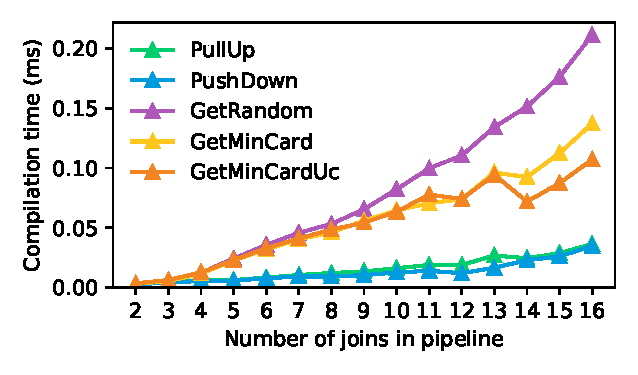
\includegraphics[width=\linewidth]{figures/2_2_enumeration_timings.pdf}
        \vspace{-0.65cm}
        \caption{Average Pipeline Compilation Time [ms] for Different Join Order Selection Strategies on SSB.}
				\label{fig:2_2_enumeration_timings}
    \end{minipage}
		\vspace{-0.5cm}
\end{figure}

\begin{figure*}[!t]
    \centering
    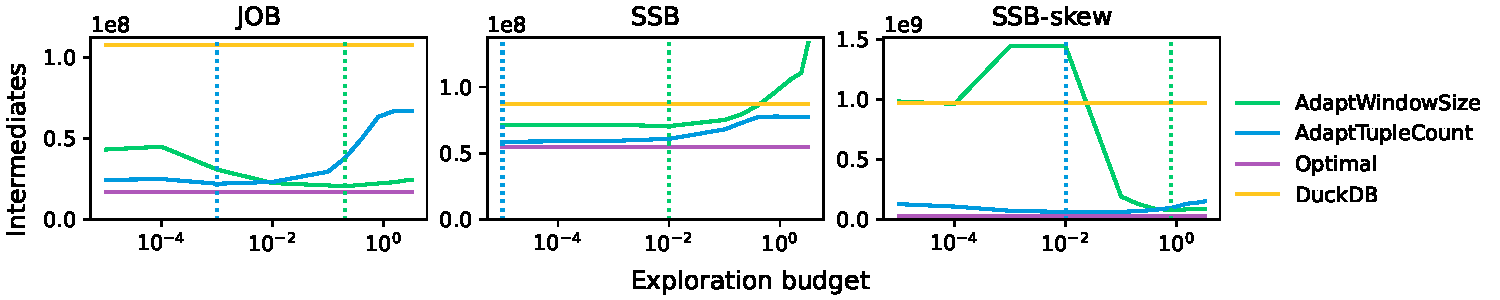
\includegraphics[width=0.95\textwidth]{figures/2_3_routing_adaptive.pdf}
		\vspace{-0.25cm}
    \caption{Exploration Budgets -- Number of Intermediate Tuples for Different Routing Strategies and Exploration Budgets (the dotted lines denote sweet spots in which the strategy generates minimal intermediates).}
    \label{fig:2_3_routing_adaptive}
		\vspace{-0.2cm}
\end{figure*}

In order to understand the trade-offs of different join selection and routing strategies, in a second series of experiments, we conduct several micro benchmarks regarding plan quality, compilation time, adaptivity, and runtime overhead. We also investigate the impact of the exploration budget on adaptivity and overhead. All micro benchmarks were executed single-threaded to isolate the effects.

\textbf{Sampling for Join Order Selection:} The \textsc{SelSampling} join selection strategy---introduced in Section~\ref{sec:paths}---systematically samples the space of cardinalities to find alternative join orders. We set the maximum join order count ${MAX}$ to $\card{J}!$ (\ie the number of possible orders for joins $J$, assuming clique queries). For an increasing number of samples, we determine the best possible outcome for the resulting join order set in terms of the intermediate optimum introduced in Section~\ref{sec:potential-analysis}. As a baseline, we exhaustively enumerate all possible join orders for each of the join pipelines. The results in Figure~\ref{fig:2_0_sample_size} show that even few samples allow for effective intermediate result reduction close to the level of exhaustive enumeration. By default, we set the sample count to 8 for the following experiments, which allows POLAR to find well-performing sequences of join paths while excluding unnecessary routing options. We used SSB-skew to test performance penalties induced by exhaustive enumeration and found deteriorations---despite no very long join pipelines---of up to 9\,\% with \textsc{AdaptTupleCount} and 1.5\,\% with \textsc{AdaptWindowSize} compared to \textsc{SelSampling} using 8 samples.

\textbf{Pipeline Compilation Time:} The time required to compile a POLAR pipeline is dominated by the join order selection. We measure this compilation time for the different join order selection strategies using pipelines with varying numbers of joins from SSB and SSB-skew as they contain the longest join pipelines. Figure~\ref{fig:2_2_enumeration_timings} compares the average pipeline compilation time with an increasing number of samples for \textsc{SelSampling} to the other strategies (again, with a join path limit of 8). Our results show that \textsc{SelSampling} generally takes longer to compile than the baselines, and its compilation time increases linearly until it reaches 8 join orders. After that, the increase becomes smaller as the strategy stops taking new samples if we already found $MAX$ distinct join orders. In any case, the compilation time for any pipeline is way below one millisecond and thus, negligible compared to the overall query processing times.

\begin{table}[!t]
  \centering
  \caption{Join Order Selection -- Total number of intermediates for POLAR pipelines with different selection strategies.}
  \vspace{-0.3cm}  \setlength\tabcolsep{3.5pt}
  \begin{tabular}{lrrrr}
    \toprule
    \textbf{Enumeration} & \textbf{JOB} & \textbf{SSB} & \textbf{SSB-skew} & \textbf{JOB-ldt}\\
    \midrule
    DuckDB* &     107.49 M &      87.36 M &     967.78 M &     248.30 M\\
    Optimal &      16.92 M &      55.06 M &      25.15 M & N/A\\
    \midrule
    \textsc{GetRandom} &      16.92 M &      55.06 M &      25.15 M &     156.64 M\\
    \textsc{GetMinCard} &      16.92 M &      55.06 M &      25.15 M &     189.47 M\\
    \textsc{GetMinCardUc} &      16.92 M &      55.06 M &      25.15 M &     189.44 M\\
    \textsc{PushDown} &      17.04 M &      59.78 M &      41.46 M &     208.83 M\\
    \textsc{PullUp} &      17.22 M &      59.88 M &      53.08 M &     210.73 M\\
    \bottomrule
  \end{tabular}
  \label{tab:1_1_sel_intms}
\end{table}


\textbf{Join Order Selection:} We further compare the quality of the join order selection strategies by comparing the actual number of intermediates to the optimal number, as described in Section~\ref{sec:potential-analysis}. To stress-test the different join order selection strategies, we also compared \textit{JOB-ldt}, which compiles the JOB queries using a greedy algorithm that only generates left-deep trees. Table~\ref{tab:1_1_sel_intms} summarizes the results.
For \textsc{GetMinCard} and \textsc{GetRandom}, we limit the number of join orders to 8, analogous to the \textsc{SelSampling}. For our set of benchmarks, even simple strategies such as \textsc{PushDown} yield competitive results that are close to the optimal number of intermediates. However, especially on SSB-skew, \textsc{PullUp} performs poorly. On JOB-ldt, \textsc{SelSampling} outperforms our baselines noticeably. Furthermore, as \textsc{GetMinCard} and \textsc{GetRandom} always produce the maximal number of join orders within the user-set limit and \textsc{PushDown} may include plans that are highly unlikely well-performing (such as an PK-FK join on a table without predicate as first join), \textsc{SelSampling} is the only strategy that may select small sets of useful, complementary join orders excluding unreasonable join paths. Therefore, we use \textsc{SelSampling} as POLAR's default.

\textbf{Join Order Initialization:} All routing strategies (excluding \textsc{Backpressure}) use a static number of tuples to initialize each of the join paths. In \textsc{AdaptWindowSize}, this number is also used to explore weaker paths after the initialization phase. To find a meaningful tuple count for path (re-)initialization, we conduct an experiment using the \textsc{InitOnce} strategy with an increasing number of initialization tuples and count the resulting number of intermediates. Figure~\ref{fig:2_5_init_tuple}  shows the results of that experiment. For JOB, 8 initialization tuples are already sufficient to determine join orders that produce less than 40\,\% intermediates incurred by DuckDB. However, for SSB, the number of intermediates gradually improves with the number of tuples. Therefore, we conservatively set the default initialization tuple count to 1024, which is also the chunk size in our DuckDB-based prototype.

\begin{figure}[!t]
    \centering
    \includegraphics[width=0.9\linewidth]{figures/2_5_init_tuple.pdf}
		\vspace{-0.5cm}
    \caption{Path Initialization -- Relative Number of Intermediates for Initial Input Tuple Counts using InitOnce.}
    \label{fig:2_5_init_tuple}
		\vspace{-0.5cm}
\end{figure} 

\textbf{Exploration Budgets:} For adaptive routing strategies, such as \textsc{AdaptTupleCount} and \textsc{AdaptWindowSize}, the quality of routing depends on the exploration budget. A higher budget allows the strategies to adapt better to path changes but also incurs larger overheads. To understand how the exploration budget affects the different workload characteristics, we execute JOB, SSB, and SSB-skew with exploration budgets from 0.001\,\% to 320\,\%. Figure \ref{fig:2_3_routing_adaptive} shows how the number of intermediates produced by the two adaptive routing strategies varies with increasing exploration budget. Both \textsc{AdaptTupleCount} and \textsc{AdaptWindowSize} achieve close to the optimal numbers of intermediates. However, the ideal exploration budgets differ for each benchmark. We attribute this effect to the differences in exploration potential, already observed in \ref{sec:potential-analysis}. 
%
While a larger budget only creates exploration overhead for SSB, exploration is crucial to find better join order alternatives for JOB and SSB-skew as the data characteristics change during query execution. \textsc{AdaptWindowSize} is especially sensitive to the exploration budget while \textsc{AdaptTupleCount} shows more robust behavior: small exploration budgets of up to 1\,\% are sufficient to obtain robust performance characteristics. Moreover, the sweet spots for \textsc{AdaptWindowSize} are generally higher than for \textsc{AdaptTupleCount} as the latter consistently keeps exploring alternative join orders even under small exploration budgets. As a result of this analysis, we set the exploration budget for \textsc{AdaptWindowSize} to 1\,\% and \textsc{AdaptTupleCount} to 0.1\,\% for the following experiments.

\begin{table}[!t]
	\centering
	\caption{Intermediate Results -- Total number of intermediates per routing strategy using tuned exploration budgets.}
	\vspace{-0.3cm} \setlength\tabcolsep{7.9pt}
  \begin{tabular}{lrrr}
	\toprule
		\textbf{Routing Strategy} & \textbf{JOB} & \textbf{SSB} & \textbf{SSB-skew}\\
		\midrule
		DuckDB &     107.49 M &      86.65 M &     929.87 M\\
		Optimal &      17.01 M &      55.06 M &      25.15 M\\
        \midrule
		\textsc{InitOnce} &      43.27 M &      67.84 M &     985.83 M\\
		\textsc{Opportunistic} &      24.48 M &      58.71 M &     655.38 M\\
		\textsc{AdaptTupleCount} &      22.05 M &      \textbf{58.70 M} &      \textbf{62.93 M}\\
		\textsc{AdaptWindowSize} &      \textbf{20.51 M} &      70.53 M &     77.92 M\\
		\textsc{Backpressure} &      41.94 M &     227.33 M &     651.14 M\\
		\bottomrule
	\end{tabular}
	\label{tab:2_4_routing_all}
\end{table}


\textbf{Routing Strategies -- Intermediates:} We compare the different routing strategies from Section~\ref{sec:routing_strategies} with regard to the number of intermediates they produce. Table~\ref{tab:2_4_routing_all} shows the results. \textsc{AdaptTupleCount} produces the least intermediates for JOB and shows competitive performance for SSB, whereas \textsc{AdaptWindowSize} produces the fewest intermediate results for SSB-Skew. \textsc{InitOnce} performs substantially worse than the adaptive strategies because it picks sub-optimal join orders whenever the initialization phase is not representative for the remaining data batches. This observation is especially pronounced for SSB-skew, where there are different optimal plans for different clusters of the data. The \textsc{Opportunistic} strategy performs best on SSB as it allows path switching without the overhead of exploration. \textsc{Backpressure} produces the most intermediate results because many executor threads process tuples through sub-optimal join orders.

\begin{table}[!t]
	\centering
	 \caption{Execution Time -- Total pipeline execution time per routing strategy [seconds].}
	 \vspace{-0.3cm}  \setlength\tabcolsep{11.4pt}
   \begin{tabular}{lrrr}
	  \toprule
		\textbf{Routing strategy} & \textbf{JOB} & \textbf{SSB} & \textbf{SSB-skew}\\
		\midrule
		DuckDB &      49.42 &       5.56 &      11.94\\
		\midrule
		\textsc{InitOnce} &      32.38 &       5.12 &      10.44\\
		\textsc{Opportunistic} &      31.44 &       6.78 &       9.40\\
		\textsc{AdaptTupleCount} &      31.44 &       7.46 &       6.50\\
		\textsc{AdaptWindowSize} &      31.02 &       5.21 &       5.36\\
		\textsc{Backpressure} &      68.35 &      14.26 &      20.65\\
		\bottomrule
	\end{tabular}
	\label{tab:3_1_pipeline}
\end{table}


\textbf{Routing Strategies -- Execution Time:} The performance of routing strategies does not solely depend on reducing intermediates. Another influential factor is how much adaptivity negatively affects vectorized execution. A high path switching rate can reduce intermediate buffer sizes, as explained in Section~\ref{sec:routing_strategies}. Therefore, we also examine the actual pipeline execution times for each routing strategy, as they are closely correlated with overall query execution time. Table \ref{tab:3_1_pipeline} shows the total pipeline execution time for different strategies using the tuned exploration budgets reported before. Since \textsc{AdaptWindowSize} trades path exploration granularity for better vectorization, the strategy performs best for exploration budgets that are below its sweet spots for minimal intermediates. Interestingly, the lowest number of intermediates does not necessarily lead to the lowest pipeline execution time. 
Despite producing more intermediates than its competitors on JOB and SSB, \textsc{AdaptWindowSize} outperforms each of them in all of our benchmarks. Therefore, we conclude that the strategy offers the best trade-off between reducing the number of intermediates and preserving good vectorized execution. Thus, we use \textsc{AdaptWindowSize} as POLAR's default routing strategy for the remainder of the experiments.

\begin{figure*}[!t]
    \centering
    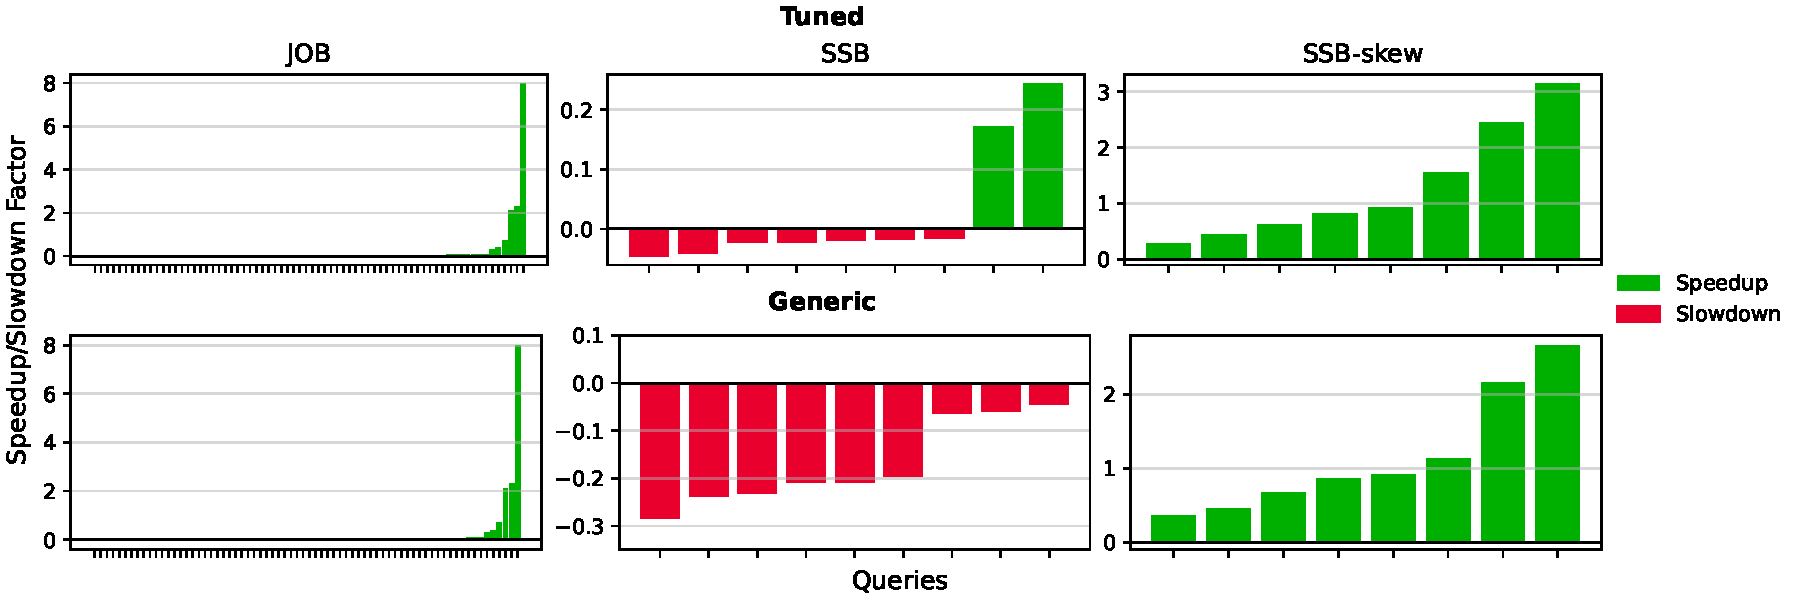
\includegraphics[width=0.99\textwidth]{figures/3_2_rel_gains.pdf}
    \vspace{-0.25cm}
    \caption{Individual Query Performance Impact -- Query performance changes between unmodified DuckDB and POLAR. A value of +1 indicates the query was 100\,\% faster (2x), and a value of -1 indicates a 100\,\% overhead (doubled execution time).}
    \label{fig:3_2_rel_gains}
		\vspace{-0.1cm}
\end{figure*}

\subsection{End-to-End Performance Comparison}
\label{sec:end-to-end}

Informed by the results from our micro benchmarks, we evaluate POLAR's end-to-end benchmark performance with \textsc{SelSampling} join order selection with 8 samples, an initialization tuple count of 1024, and the \textsc{AdaptWindowSize} routing strategy with a 1\,\% exploration budget for all benchmarks. In this context, we compare POLAR with DuckDB~\cite{RaasveldtM19}, a Lookahead Information Passing~\cite{ZhuPSP17} prototype on DuckDB, Postgres~\cite{DBLP:conf/sigmod/StonebrakerR86}, SkinnerDB (\ie Skinner-C)~\cite{TrummerWMMJA19}, and SkinnerMT~\cite{WeiT22}, a state-of-the-art AQP system, in both single- and multi-threaded configurations.

\begin{table}
	\centering
	\caption{Overall Performance Impact -- Single-threaded total execution time, and max execution time per query [seconds].}
		\vspace{-0.3cm} \setlength\tabcolsep{3.7pt}
   \begin{tabular}{lcccccc}
	  \toprule
		& \multicolumn{3}{c}{\textbf{Total Execution Time}} & \multicolumn{3}{c}{\textbf{Max. Query Time}}\\
         & JOB & SSB & SSB-skew & JOB & SSB & SSB-skew\\
		\midrule
		DuckDB & 135.5 & 7.8 & 12.2 & 10.7 & 1.1 & 3.6\\
        POLAR-G & 117.7 & 8.9 & 5.6 & 3.9 & 1.4 & 1.7\\
        POLAR-T & \textbf{117.7} & \textbf{7.5} & \textbf{5.6} & \textbf{3.9} & \textbf{0.9} & \textbf{1.7} \\
        Speedup & 1.15x & 1.04x & \textbf{\color{red}2.18x} & \textbf{\color{red}2.74x} & 1.22x & \textbf{\color{red}2.12x}\\
		\bottomrule
	\end{tabular}
	\label{tab:3_4_endtoend}
\end{table}


\begin{figure*}
    \centering
    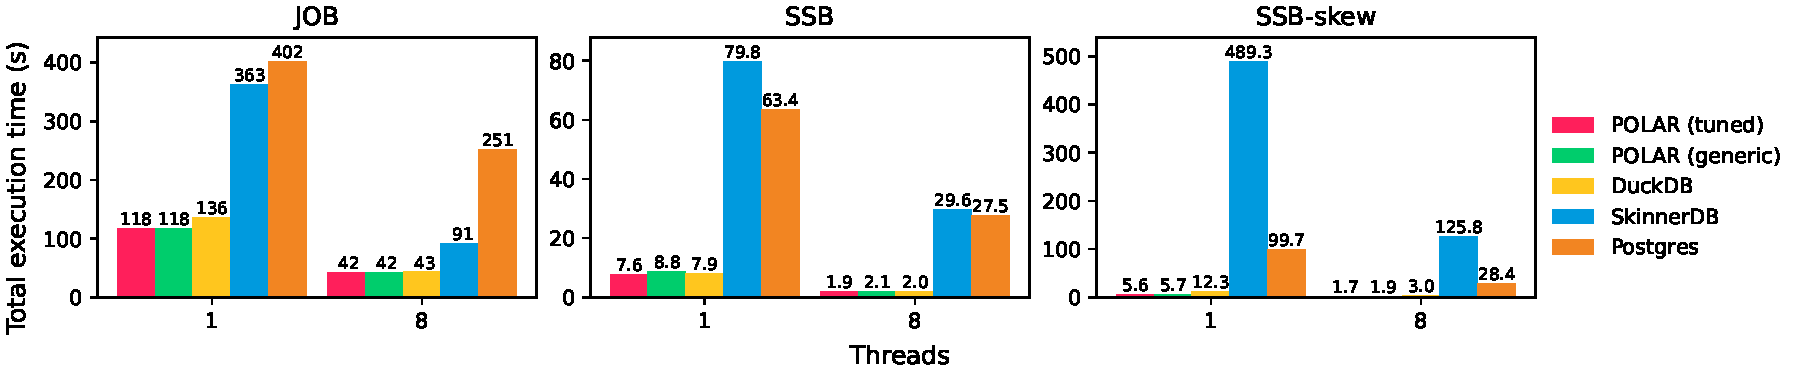
\includegraphics[width=0.99\textwidth]{figures/4_1_total.pdf}
    \vspace{-0.25cm}
    \caption{AQP System Comparison -- Total execution times for JOB, SSB, and SSB-skew, using 1 and 8 threads [seconds].}
    \label{fig:4_1_total}
		\vspace{-0.1cm}
\end{figure*}

\textbf{Overall Performance Impact:} Table~\ref{tab:3_4_endtoend} shows the total, end-to-end, single-threaded execution time and the maximum query execution times for DuckDB and POLAR on the different benchmarks. POLAR shows a slight overhead on SSB in total and maximum execution times and a moderate total execution time improvement of 1.16x on JOB. Moreover, POLAR shows a substantial 1.94x end-to-end improvement for SSB-skew and reduces the maximal query runtimes for JOB and SSB-skew by 2.78x and 2.98x, respectively. These results show that POLAR yields robust performance with substantial improvements for workloads on skewed data and only minor overhead for workloads where adaptation is not needed.

\textbf{Query Performance Impact:} Figure~\ref{fig:3_2_rel_gains} shows the speedups and slowdowns for each individual query with POLAR-amenable pipelines in JOB, SSB, and SSB-skew. A value of 1 indicates an improvement of 100\,\% (\ie half the execution time or 2x), whereas a value of -1 indicates double the execution time. For most JOB queries, POLAR has no positive or negative effect on the execution time. However, for a few queries, POLAR substantially reduces the execution time by up to 9x. The two queries with the largest speedups are also the longest-running queries in the benchmark. On SSB, the POLAR overhead increases the execution time for most queries, as expected, given how close to optimal the original plans are. However, one of the SSB queries also benefits from POLAR. Finally, almost all queries in SSB-skew improve with POLAR, up to 4x in one case. Therefore, POLAR achieves substantial performance and robustness improvements on non-uniform data and incurs only slight overhead for some queries on uniform data due to plan exploration and impact on vectorization at runtime. However, this moderate overhead is an acceptable price to pay for increased robustness, and the overhead could be further decreased when specializing POLAR to the underlying runtime system.

\textbf{Number of Intermediates:} The execution times of our baseline systems are strongly correlated with their underlying execution engines. Hence, we first conduct an experiment comparing the number of intermediates produced by their join orders. Table~\ref{tab:3_5_intermediates} shows the results. Note that SkinnerDB ran out-of-memory for SSB and SSB-skew. However, for JOB, SkinnerDB achieves a much lower number of intermediates than DuckDB, POLAR, and Postgres because it is not restricted to amenable pipelines. The comparison further shows that Postgres generally produces plans with fewer intermediates than DuckDB. Using POLAR reduces DuckDB's intermediates and outperforms Postgres by 1.4x on SSB-skew.

\input{tables/3_5_intermediates}

\textbf{AQP System Comparison:} To contextualize POLAR's performance, we compare POLAR, DuckDB, Postgres, SkinnerDB, and SkinnerMT, measuring the total execution time in single- and multi-threaded (8 threads) configurations. Additionally, we implemented a prototype of Lookahead Information Passing~\cite{ZhuPSP17} (LIP) in DuckDB to compare POLAR against a bitmap filtering approach. We allow SkinnerDB/MT to cache indexes on all join columns in memory to reduce its pre-processing time. We use Postgres 12.15 with indexes on all foreign key columns to prevent it from compiling aggressive plans with fatal nested-loop joins on unindexed join columns.
%
Figure~\ref{fig:4_1_total} shows that POLAR performs equally or better than DuckDB, SkinnerDB, and Postgres on almost all benchmarks. On SSB, POLAR shows a similar performance as DuckDB both single- and multi-threaded. On SSB-skew, POLAR outperforms DuckDB by 1.9x single-threaded and by 1.8x multi-threaded.
%LIP
While LIP shows equal execution times as POLAR on JOB, it performs slightly worse on SSB and substantially worse on SSB-skew. Regarding individual JOB queries, LIP shows occasional performance regressions of more than 2x, which is in line with experimental results from other bitmap filtering approaches \cite{DingCN20, LeeDNC23}. We account this performance gap to the large number of additional hash probes, lack of vectorization, and unstable bloom filter orderings.
%SkinnerDB/MT
SkinnerMT shows the best performance on JOB with multiple threads. However, SkinnerDB/MT run out-of-memory on SSB and SSB-skew. Previous experiments on SSB with scale factor 10 showed POLAR speedups of up to 15.6x over SkinnerDB (8 threads, 1.9\,s vs 29.6\,s) and around 3.9x over SkinnerMT. We attribute this to SkinnerDB/MTs custom join operator with tuple-at-a-time processing and the systems' ability to change the source table, which requires building hash tables for each relation.
%Postgres
As expected, Postgres shows much higher total execution times than POLAR and DuckDB, given its different target workloads and runtime system. These experiments demonstrate the benefits of a non-invasive, bounded-overhead system design in an engine designed for analytic workloads. In contrast to invasive AQP systems, POLAR favors reusing existing database components and original plans resulting in competitive performance and much greater performance robustness with modest overhead.


%% RELATED WORK
\vspace{0.4cm}
\section{Related Work}
\label{related-work}
%
Besides the brief background in the introduction, here, we broadly survey related work and emphasize the differences of POLAR.

\textbf{Traditional AQP:} Adaptive query processing has received lots of attention in the data management literature, and great surveys \cite{BabuB05,DeshpandeIR07} and tutorials \cite{IvesDR07,DeshpandeHR06} already exist. Existing classifications distinguish AQP for traditional ad-hoc queries (or plan-based systems) versus continuous queries \cite{BabuB05}, as well as a spectrum of adaptivity from coarse- to fine-grained adaptation \cite{DeshpandeHR06}.
First, \emph{inter-query} optimization utilizes learned cardinalities for expressions \cite{BrunoC02,ChenR94,StillgerLMK01} for optimizing future queries. Second, \emph{inter-pipeline} optimization utilizes monitored statistics even within a single query. Examples are late binding (staged execution) with re-optimization at pipeline breakers \cite{DeshpandeHR06} or at parameter binding in parametric query optimization \cite{BizarroBD09}. Third, \emph{inter-operator} re-optimization compiles new remaining plans at so-called checkpoint operators \cite{KabraD98}. Similar, progressive and pro-active re-optimization apply plan changes if actual cardinalities are outside computed validity ranges \cite{MarklRSLP04,BabuBD05}. Fourth, \emph{intra-operator} adaptivity allows changing plans after partial operator evaluation. Examples are union stitch-up plans and handling of state in double-pipelined hash joins \cite{IvesHW04}, intra-query adaptivity via reinforcement learning in SkinnerDB \cite{TrummerWMMJA19,TrummerWWMMJAR21,WeiT22}, as well as adaptive join reordering of index-nested-loop joins with depleted states for correctness \cite{LiSMBCL07}. Fifth, there is tuple routing with routing policies in Eddies~\cite{HellersteinA00,Arpaci-Dusseau03,Deshpande04,BizarroBDW05}. Many of these strategies require both optimizer and runtime extensions for effective and efficient adaptivity. Moreover, Eddies requires complex tuple tracking to produce correct results. Instead, POLAR aims at a simple system integration with bounded exploration overhead.

\textbf{AQP for Continuous Queries:} The adaptation of continuous queries---on infinite data streams---always focuses on \emph{intra-operator} and \emph{tuple-routing}. Early stream processing systems with adaptive query processing include STREAM \cite{BabuW04}, Aurora \cite{AbadiCCCCLSTZ03}/Borealis~\cite{AbadiABCCHLMRRTXZ05}, NiagaraCQ \cite{ChenJDTW00}, and TelegraphCQ \cite{ChandrasekaranDFHHKMRRS03}. Unique characteristics are the incremental collection of statistics to detect workload changes \cite{BabuMMNW04}, multi-query optimization with queries entering and leaving the system, asynchronous optimization outside the critical path \cite{Boehm2011}, the applicability of load shedding \cite{TatbulCZCS03}, as well as stateful operators and queues which require draining for plan changes \cite{WangFMWZ19}. Modern distributed stream processing engines like Flink \cite{AlexandrovBEFHHKLLMNPRSSHTW14}, Spark \cite{ZahariaDLHSS13}, Beam \cite{AkidauBCCFLMMPS15}, Heron~\cite{KulkarniBFKKMPR15}/Dhalion~\cite{FloratouAGRR17}, and NebulaStream \cite{ZeuchCMGGGBTM20} further deal with the reconfiguration of distributed query topologies. In contrast to POLAR, AQP is naturally deeply integrated in almost all components of such stream processing engines.

\textbf{Different Plans for Different Data:} Both, ad-hoc and continuous queries are typically compiled and optimized according to average statistics. However, especially in correlated data, relations are naturally divided into partitions with different characteristics \cite{TzoumasDJ10}. Early work on selectivity-based partitioning \cite{Polyzotis05} and content-based routing \cite{BizarroBDW05} address this observation by generating different plans for different partitions, and different value-based routing policies. Such approaches often leverage more fine-grained statistics such as serial histograms (i.e., detailed frequency matrices) \cite{Ioannidis93}. Recent work on multi-way join size estimation \cite{MullerM22,IzenovDRS21} utilize hash-based translation grids \cite{MullerM22} and AKMV sketches \cite{BeyerHRSG07} as well as fast-AGMS sketches \cite{IzenovDRS21}. Since selectivity-based partitioning might compute the same intermediate multiple times, further work on sharing-aware horizontal partitioning \cite{TzoumasDJ10} introduced a conditional join plan, and related optimization and runtime techniques. Exploratory AQP via reinforcement learning like SkinnerDB~\cite{TrummerWMMJA19} would also lend itself to discovering different paths. Due to repeated path sampling, POLAR can also exploit different paths for different data, but only if these tuples are scanned in a clustered manner.

\textbf{Micro Adaptivity:} Besides finding alternative plans (e.g., join orders), some work also focused on micro adaptivity. Raducanu et al. introduced this concept in Vectorwise \cite{RaducanuBZ13} by providing alternative kernel implementations (e.g., branch, no-branch), measuring their runtime on sample vectors, and selecting the best configuration via a learning algorithm. Later work used performance counters to minimize the measurement overhead, and more properties such as sortedness and co-clustering \cite{ZeuchPF16}. Other forms of micro adaptivity are compiling continuous queries for HW specialization, parallelization, as well as exploitation of selectivities or value distributions \cite{GrulichBZTBCRM20,RosenfeldBM23}. Micro adaptivity requires specific optimization algorithms, whereas POLAR relies on existing optimizers without changes. 

\textbf{AQP for Non-relational Workloads:} AQP ideas have also been applied and extended for non-relational systems and workloads. Examples include JIT compilation for programming languages~\cite{HolzleU94} (e.g., Java or WebAssembly); lazy expression compilation in TensorFlow~\cite{MoldovanDWJLNSR19}, dynamic recompilation of blocks and functions in SystemML~\cite{BoehmBERRSTT14}; periodic or on-demand reoptimization of integration flows \cite{Boehm2011}; and AQP on raw data \cite{KarpathiotakisBAA14}. These systems also incrementally collect telemetry and perform plan adaptation, but unlike POLAR, seek a single optimal plan or configuration. 

\textbf{Learned Optimizers and Estimators:} With the trend towards ML for systems \cite{KraskaBCDP18}, there has been substantial progress on improved cardinality estimates that could mitigate some of the need for AQP. Early work focused on the featurization of schemas and workloads and sampling-based training data collection \cite{KipfKRLBK19,DuttWNKNC19,YangLKWDCAHKS19}. Hilprecht and Binnig later introduced representations for zero-shot cost models \cite{HilprechtB22,HilprechtB22b} that can generalize to unseen database instances. Early work like LEO \cite{StillgerLMK01} also focused on learned cardinalities, but in retrospective had the problem of \enquote{fleeing from knowledge to ignorance} \cite{Lohman17} because the exponential search space gets only sparsely sampled,  and skewed cardinalities are often larger than the estimates under independence assumption. However, recent work has shown that learned optimizers and cardinality estimators can learn from mistakes \cite{MarcusNMZAKPT19,MarcusNMTAK21}, making a case for stateful, learning-based systems \cite{abs-2303-15308}, especially for cloud DBMS like Snowflake \cite{DagevilleCZAABC16} or Redshift \cite{GuptaATKPSS15}. In contrast to POLAR, integrating learned optimizers and estimators is still very invasive in terms of system complexity, bootstrapping, and integration points.


%% CONCLUSIONS
\section{Conclusions}
% summary
We introduced the new concept of plans of least resistance for leveraging adaptive query processing in a non-invasive manner. POLAR pipelines replace, where applicable, standard join pipelines and internally multiplex tuple batches among alternative join paths. This design allows periodically sampling join paths, collecting telemetry, and adapting the routing to the best path accordingly. 
% conclusions
We draw three key conclusions. First, the simple design without optimizer changes greatly simplified the integration into systems such as DuckDB. Second, POLAR shows robust performance but only on workloads yielding a large fraction of applicable pipelines. Third, there are examples of substantial performance improvements for individual pipelines, queries, and workloads, especially for skewed data (fix for bad cardinality estimates) and clustered data (exploit different plans for different data partitions).
% future work
Interesting directions of future work include more advanced strategies for selecting alternative pipelines (e.g., considering the uncertainty of cardinality estimates), and broader support for different plan structures (e.g., DAGs, bushy plans, additional operators like groupjoin \cite{MoerkotteN11}). 


\begin{acks}
We thank the participants of Dagstuhl Seminar 17222~\cite{DBLP:journals/dagstuhl-reports/Borovica-GajicG17} and 22111~\cite{DBLP:journals/dagstuhl-reports/Borovica-GajicG22} for inspiring this research and invaluable discussions. We also gratefully acknowledge funding from the German Federal Ministry of Education and Research (under research grant BIFOLD23B) as well as initial funding from SAP.
\end{acks}

%\clearpage
\balance
\bibliographystyle{ACM-Reference-Format}
\bibliography{sample-base_new}

\end{document}
\endinput
